\documentclass{standalone}
\usepackage{tikz}
\usetikzlibrary{patterns}
\usetikzlibrary{positioning}
\usetikzlibrary{patterns, positioning}
\usetikzlibrary{shapes.misc}
\usepackage[outline]{contour}
\contourlength{1.5pt} 
\usepackage[sfdefault]{ClearSans}

\begin{document}
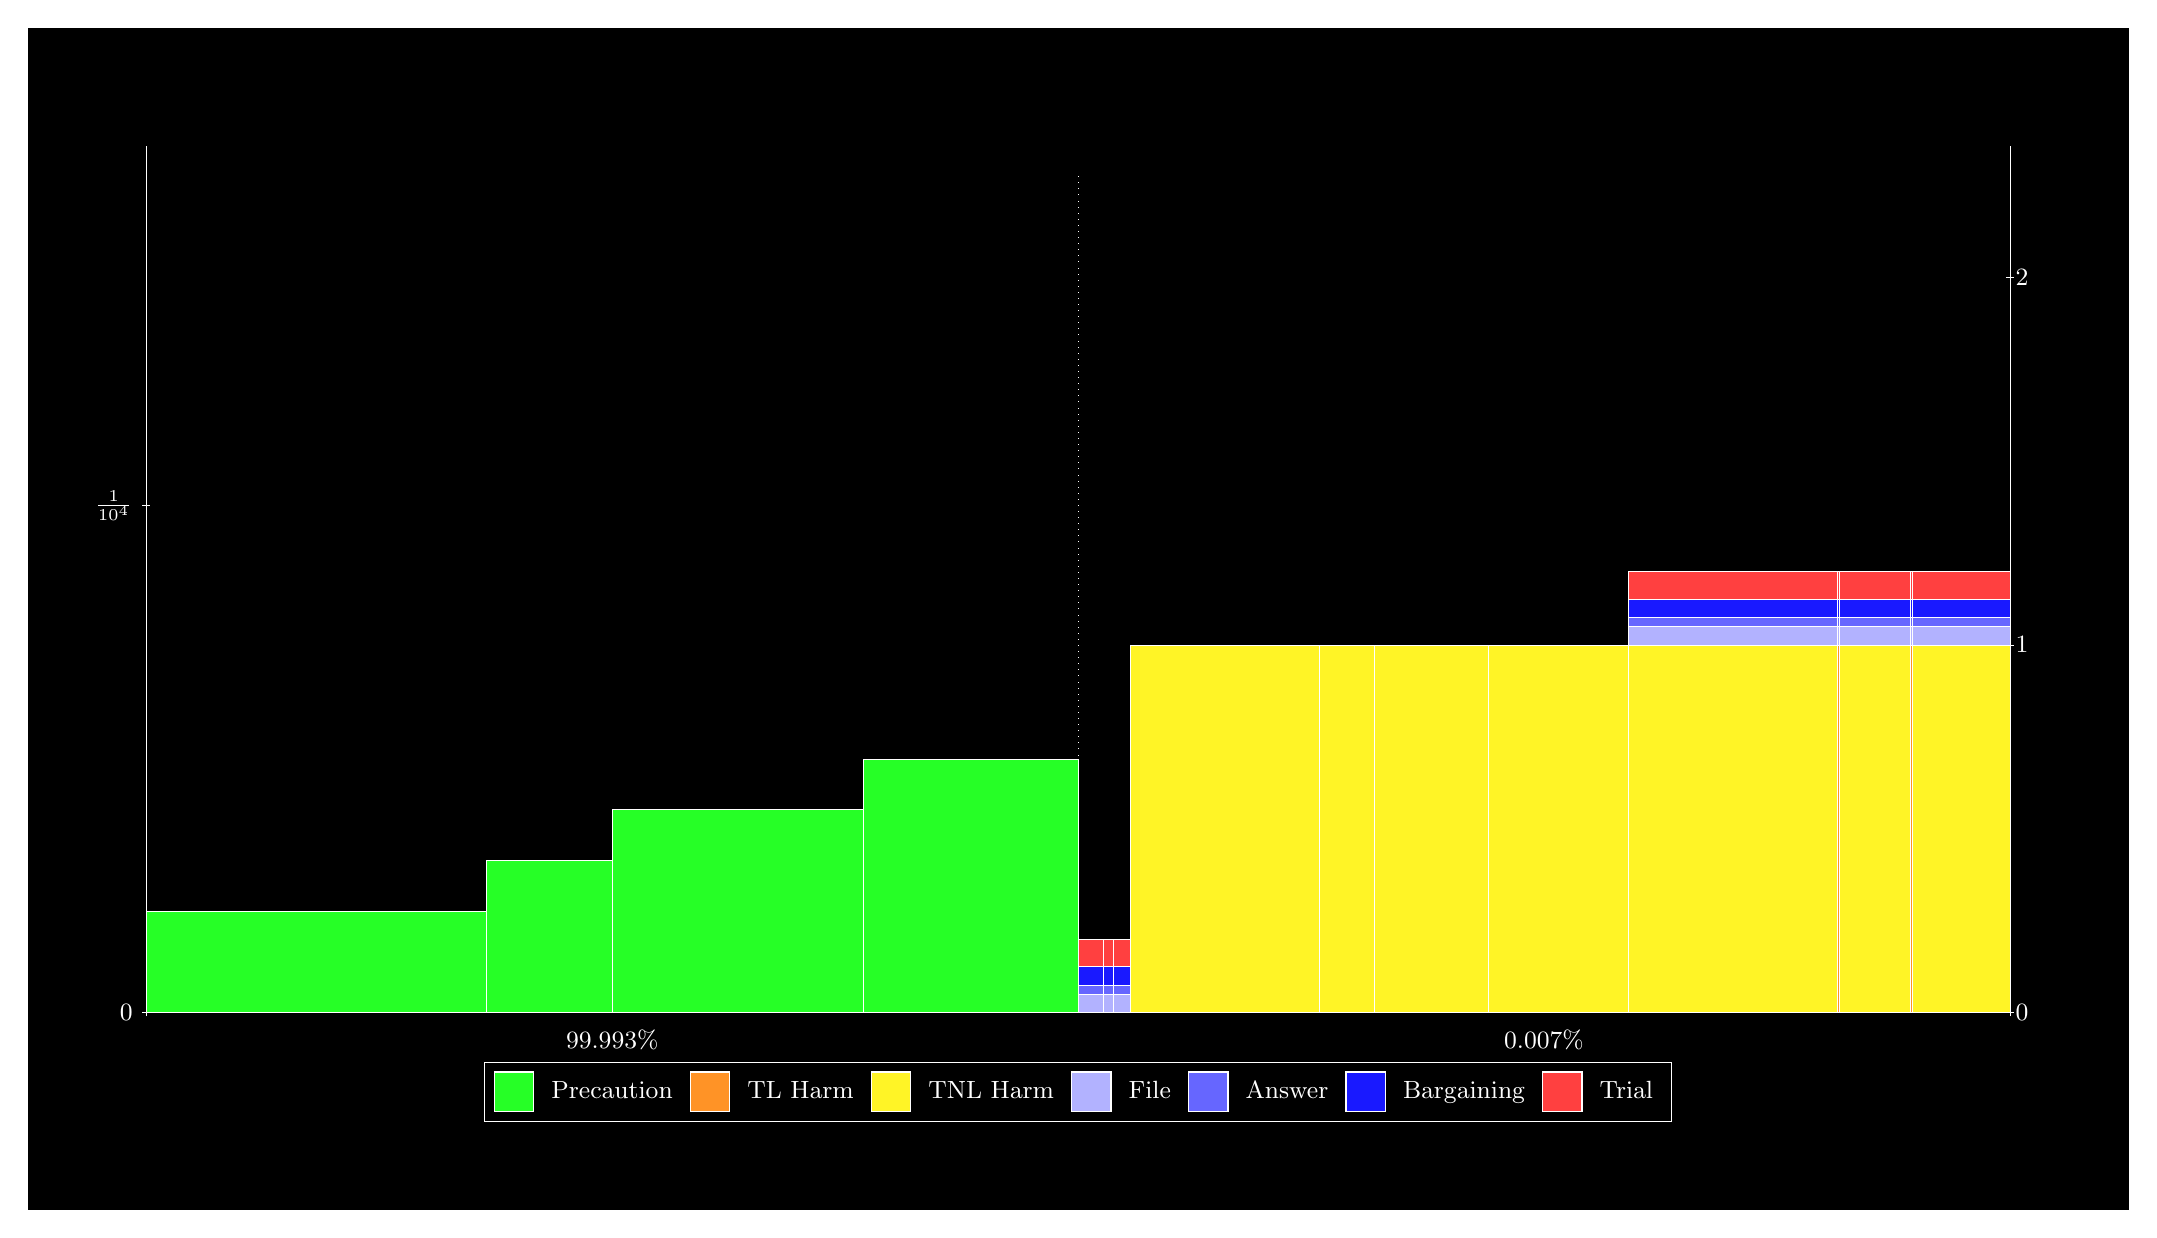
\begin{tikzpicture}
\draw[fill=black] (0,0) rectangle (26.667,15);
\draw[fill=green!85,draw=white,very thin] (1.5,2.5) rectangle (5.8205,3.7872);
\draw[fill=green!85,draw=white,very thin] (5.8205,2.5) rectangle (7.4166,4.4309);
\draw[fill=green!85,draw=white,very thin] (7.4166,2.5) rectangle (10.611,5.0745);
\draw[fill=green!85,draw=white,very thin] (10.611,2.5) rectangle (13.333,5.7181);
\draw[fill=green!85,draw=white,very thin] (13.333,2.5) rectangle (13.652,2.5001);
\draw[fill=blue!30,draw=white,very thin] (13.333,2.5001) rectangle (13.652,2.7336);
\draw[fill=blue!60,draw=white,very thin] (13.333,2.7336) rectangle (13.652,2.8503);
\draw[fill=blue!90,draw=white,very thin] (13.333,2.8503) rectangle (13.652,3.0838);
\draw[fill=red!75,draw=white,very thin] (13.333,3.0838) rectangle (13.652,3.434);
\draw[fill=green!85,draw=white,very thin] (13.652,2.5) rectangle (13.782,2.5001);
\draw[fill=blue!30,draw=white,very thin] (13.652,2.5001) rectangle (13.782,2.7336);
\draw[fill=blue!60,draw=white,very thin] (13.652,2.7336) rectangle (13.782,2.8503);
\draw[fill=blue!90,draw=white,very thin] (13.652,2.8503) rectangle (13.782,3.0838);
\draw[fill=red!75,draw=white,very thin] (13.652,3.0838) rectangle (13.782,3.434);
\draw[fill=green!85,draw=white,very thin] (13.782,2.5) rectangle (14,2.5002);
\draw[fill=blue!30,draw=white,very thin] (13.782,2.5002) rectangle (14,2.7337);
\draw[fill=blue!60,draw=white,very thin] (13.782,2.7337) rectangle (14,2.8504);
\draw[fill=blue!90,draw=white,very thin] (13.782,2.8504) rectangle (14,3.0839);
\draw[fill=red!75,draw=white,very thin] (13.782,3.0839) rectangle (14,3.4341);
\draw[fill=green!85,draw=white,very thin] (14,2.5) rectangle (16.392,2.5001);
\draw[fill=yellow!85,draw=white,very thin] (14,2.5001) rectangle (16.392,7.1694);
\draw[fill=green!85,draw=white,very thin] (16.392,2.5) rectangle (17.089,2.5001);
\draw[fill=yellow!85,draw=white,very thin] (16.392,2.5001) rectangle (17.089,7.1695);
\draw[fill=green!85,draw=white,very thin] (17.089,2.5) rectangle (18.541,2.5002);
\draw[fill=yellow!85,draw=white,very thin] (17.089,2.5002) rectangle (18.541,7.1695);
\draw[fill=green!85,draw=white,very thin] (18.541,2.5) rectangle (20.326,2.5002);
\draw[fill=yellow!85,draw=white,very thin] (18.541,2.5002) rectangle (20.326,7.1696);
\draw[fill=green!85,draw=white,very thin] (20.326,2.5) rectangle (22.973,2.5001);
\draw[fill=yellow!85,draw=white,very thin] (20.326,2.5001) rectangle (22.973,7.1694);
\draw[fill=blue!30,draw=white,very thin] (20.326,7.1694) rectangle (22.973,7.4029);
\draw[fill=blue!60,draw=white,very thin] (20.326,7.4029) rectangle (22.973,7.5196);
\draw[fill=blue!90,draw=white,very thin] (20.326,7.5196) rectangle (22.973,7.7531);
\draw[fill=red!75,draw=white,very thin] (20.326,7.7531) rectangle (22.973,8.1033);
\draw[fill=green!85,draw=white,very thin] (22.973,2.5) rectangle (23,2.5001);
\draw[fill=orange!85,draw=white,very thin] (22.973,2.5001) rectangle (23,7.1694);
\draw[fill=blue!30,draw=white,very thin] (22.973,7.1694) rectangle (23,7.4029);
\draw[fill=blue!60,draw=white,very thin] (22.973,7.4029) rectangle (23,7.5196);
\draw[fill=blue!90,draw=white,very thin] (22.973,7.5196) rectangle (23,7.7531);
\draw[fill=red!75,draw=white,very thin] (22.973,7.7531) rectangle (23,8.1033);
\draw[fill=green!85,draw=white,very thin] (23,2.5) rectangle (23.905,2.5001);
\draw[fill=yellow!85,draw=white,very thin] (23,2.5001) rectangle (23.905,7.1695);
\draw[fill=blue!30,draw=white,very thin] (23,7.1695) rectangle (23.905,7.403);
\draw[fill=blue!60,draw=white,very thin] (23,7.403) rectangle (23.905,7.5197);
\draw[fill=blue!90,draw=white,very thin] (23,7.5197) rectangle (23.905,7.7532);
\draw[fill=red!75,draw=white,very thin] (23,7.7532) rectangle (23.905,8.1034);
\draw[fill=green!85,draw=white,very thin] (23.905,2.5) rectangle (23.928,2.5001);
\draw[fill=orange!85,draw=white,very thin] (23.905,2.5001) rectangle (23.928,7.1695);
\draw[fill=blue!30,draw=white,very thin] (23.905,7.1695) rectangle (23.928,7.403);
\draw[fill=blue!60,draw=white,very thin] (23.905,7.403) rectangle (23.928,7.5197);
\draw[fill=blue!90,draw=white,very thin] (23.905,7.5197) rectangle (23.928,7.7532);
\draw[fill=red!75,draw=white,very thin] (23.905,7.7532) rectangle (23.928,8.1034);
\draw[fill=green!85,draw=white,very thin] (23.928,2.5) rectangle (25.167,2.5002);
\draw[fill=yellow!85,draw=white,very thin] (23.928,2.5002) rectangle (25.167,7.1695);
\draw[fill=blue!30,draw=white,very thin] (23.928,7.1695) rectangle (25.167,7.403);
\draw[fill=blue!60,draw=white,very thin] (23.928,7.403) rectangle (25.167,7.5197);
\draw[fill=blue!90,draw=white,very thin] (23.928,7.5197) rectangle (25.167,7.7532);
\draw[fill=red!75,draw=white,very thin] (23.928,7.7532) rectangle (25.167,8.1034);
\draw[white,very thin] (1.5,2.5) -- (1.5,13.5);
\draw[white,very thin] (1.45,2.5) -- (1.55,2.5);
\node[font=\small,text=white, anchor=east] at (1.45, 2.5) {0};
\draw[white,very thin] (1.45,8.9362) -- (1.55,8.9362);
\node[font=\small,text=white, anchor=east] at (1.45, 8.9362) {$\frac{1}{10^{4}}$};

\draw[white,dotted,very thin] (13.333,2.83) -- (13.333,13.17);
\draw[white,very thin] (25.167,2.5) -- (25.167,13.5);
\draw[white,very thin] (25.117,2.5) -- (25.217,2.5);
\node[font=\small,text=white, anchor=west] at (25.117, 2.5) {0};
\draw[white,very thin] (25.117,7.1693) -- (25.217,7.1693);
\node[font=\small,text=white, anchor=west] at (25.117, 7.1693) {1};
\draw[white,very thin] (25.117,11.839) -- (25.217,11.839);
\node[font=\small,text=white, anchor=west] at (25.117, 11.839) {2};

\draw[white,very thin] (1.5,2.5) -- (25.167,2.5);
\draw[white,very thin] (1.5,2.45) -- (1.5,2.55);
\node[font=\small,text=white, anchor=north] at (1.5, 2.45) {};
\draw[white,very thin] (25.167,2.45) -- (25.167,2.55);
\node[font=\small,text=white, anchor=north] at (25.167, 2.45) {};

\node[font=\small,text=white,anchor=south] at (7.4167, 1.9) {99.993\%};
\node[font=\small,text=white,anchor=south] at (19.25, 1.9) {0.007\%};
\draw (13.3333,2.5) node (B) {};
\begin{scope}[align=center]
\matrix[scale=0.5,draw=white,below=0.5cm of B,nodes={draw},column sep=0.1cm]{
\node[rectangle,draw,minimum width=0.5cm,minimum height=0.5cm,fill=green!85]{}; & \node[draw=none,font=\small,text=white]{Precaution}; &
\node[rectangle,draw,minimum width=0.5cm,minimum height=0.5cm,fill=orange!85]{}; & \node[draw=none,font=\small,text=white]{TL Harm}; &
\node[rectangle,draw,minimum width=0.5cm,minimum height=0.5cm,fill=yellow!85]{}; & \node[draw=none,font=\small,text=white]{TNL Harm}; &
\node[rectangle,draw,minimum width=0.5cm,minimum height=0.5cm,fill=blue!30]{}; & \node[draw=none,font=\small,text=white]{File}; &
\node[rectangle,draw,minimum width=0.5cm,minimum height=0.5cm,fill=blue!60]{}; & \node[draw=none,font=\small,text=white]{Answer}; &
\node[rectangle,draw,minimum width=0.5cm,minimum height=0.5cm,fill=blue!90]{}; & \node[draw=none,font=\small,text=white]{Bargaining}; &
\node[rectangle,draw,minimum width=0.5cm,minimum height=0.5cm,fill=red!75]{}; & \node[draw=none,font=\small,text=white]{Trial}; \\\\
};\end{scope}

\end{tikzpicture}
\end{document}